% flashcards-title: Counters grouped into loops of ten with single counters
% flashcards-desc: Two outlined loops each enclose ten identical round counters arranged in two rows of five. Below the loops, five more identical counters sit alone in a row, outside any loop.
\documentclass[tikz]{standalone}
\usetikzlibrary{arrows.meta,patterns}

\definecolor{qraNavy}{HTML}{17324D}
\definecolor{qraBlue}{HTML}{2B6CB0}
\definecolor{qraGold}{HTML}{B7791F}
\definecolor{qraPale}{HTML}{EAF2F8}
\definecolor{qraGray}{HTML}{5C6773}

\tikzset{
  qra axis/.style={draw=qraNavy, line width=1.2pt},
  qra tick/.style={draw=qraNavy, line width=1pt},
  qra guide/.style={draw=qraGray, densely dashed, line width=0.8pt},
  qra counter/.style={circle, draw=qraNavy, fill=qraPale, line width=0.9pt, minimum size=7mm, inner sep=0pt},
  qra label/.style={font=\sffamily\bfseries, text=qraNavy},
  qra small label/.style={font=\sffamily, text=qraNavy},
}

\begin{document}
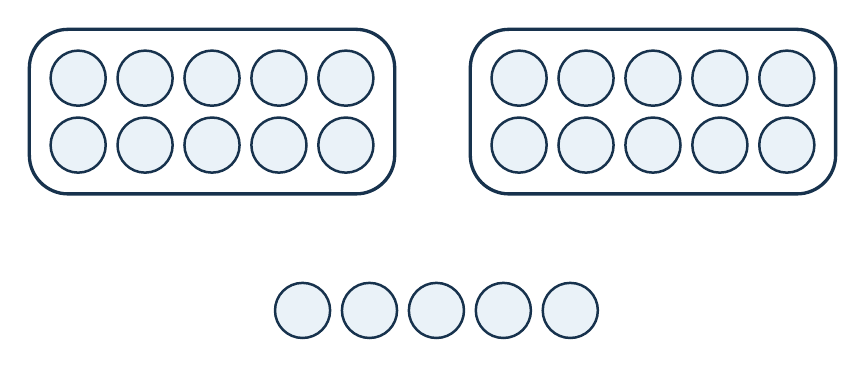
\begin{tikzpicture}
  % Loop A: ten counters in a 5 x 2 grid
  \foreach \i in {0,...,4} {
    \foreach \j in {0,1} {
      \node[qra counter] at (\i*0.85, \j*0.85) {};
    }
  }
  \draw[qra axis, rounded corners=14pt] (-0.62,-0.62) rectangle (4.02,1.47);

  % Loop B: ten counters in a 5 x 2 grid
  \begin{scope}[xshift=5.6cm]
    \foreach \i in {0,...,4} {
      \foreach \j in {0,1} {
        \node[qra counter] at (\i*0.85, \j*0.85) {};
      }
    }
    \draw[qra axis, rounded corners=14pt] (-0.62,-0.62) rectangle (4.02,1.47);
  \end{scope}

  % Five single counters outside any loop
  \foreach \i in {0,...,4} {
    \node[qra counter] at (2.85 + \i*0.85, -2.1) {};
  }
\end{tikzpicture}
\end{document}
